% Resultados -- RQ 01 a RQ 04 (parte do João).
% Números de resultados/rq1_rq4_*.csv (python -m analises.rq1_rq4_descritiva) e dos
% intervalos de resultados/ic_bootstrap.csv (python -m analises.ic_bootstrap).

Como as distribuições são assimétricas e têm cauda longa, reportamos mediana e IQR. Para
saber o quanto cada número é estável, calculamos também intervalos de confiança de 95\% por
\textit{bootstrap} percentil (2.000 reamostragens dos repositórios, semente fixa) para as
medianas, as correlações e as proporções de mudança de categoria
(Tabela~\ref{tab:descritiva}).

\begin{table}[ht]
\centering
\caption{Estatística descritiva das métricas DORA (350 repositórios) e IC 95\% da mediana.}
\label{tab:descritiva}
\footnotesize
\setlength{\tabcolsep}{4pt}
\begin{tabular}{lrrrrrc}
\hline
\textbf{Métrica} & \textbf{n} & \textbf{Q1} & \textbf{Mediana} & \textbf{Q3} & \textbf{IQR} &
\textbf{IC 95\% da mediana} \\
\hline
Frequência (releases/semana) & 350 & 0,19 & 0,42 & 1,04 & 0,84 & [0,35; 0,46] \\
Lead time (a) (h)            & 350 & 50,8 & 251,7 & 848,4 & 797,6 & [196,7; 337,3] \\
Lead time (b) (h)            & 350 & 65,4 & 284,0 & 845,4 & 780,1 & [206,8; 331,6] \\
CFR (a), proxy de CI         & 350 & 0,021 & 0,049 & 0,121 & 0,100 & [0,041; 0,065] \\
CFR (b), proxy de entrega    & 350 & 0,052 & 0,200 & 0,416 & 0,364 & [0,174; 0,227] \\
Recuperação (h)              & 330 & 0,98 & 2,56 & 9,53 & 8,55 & [2,08; 3,30] \\
\hline
\end{tabular}
\end{table}

\begin{figure}[ht]
\centering
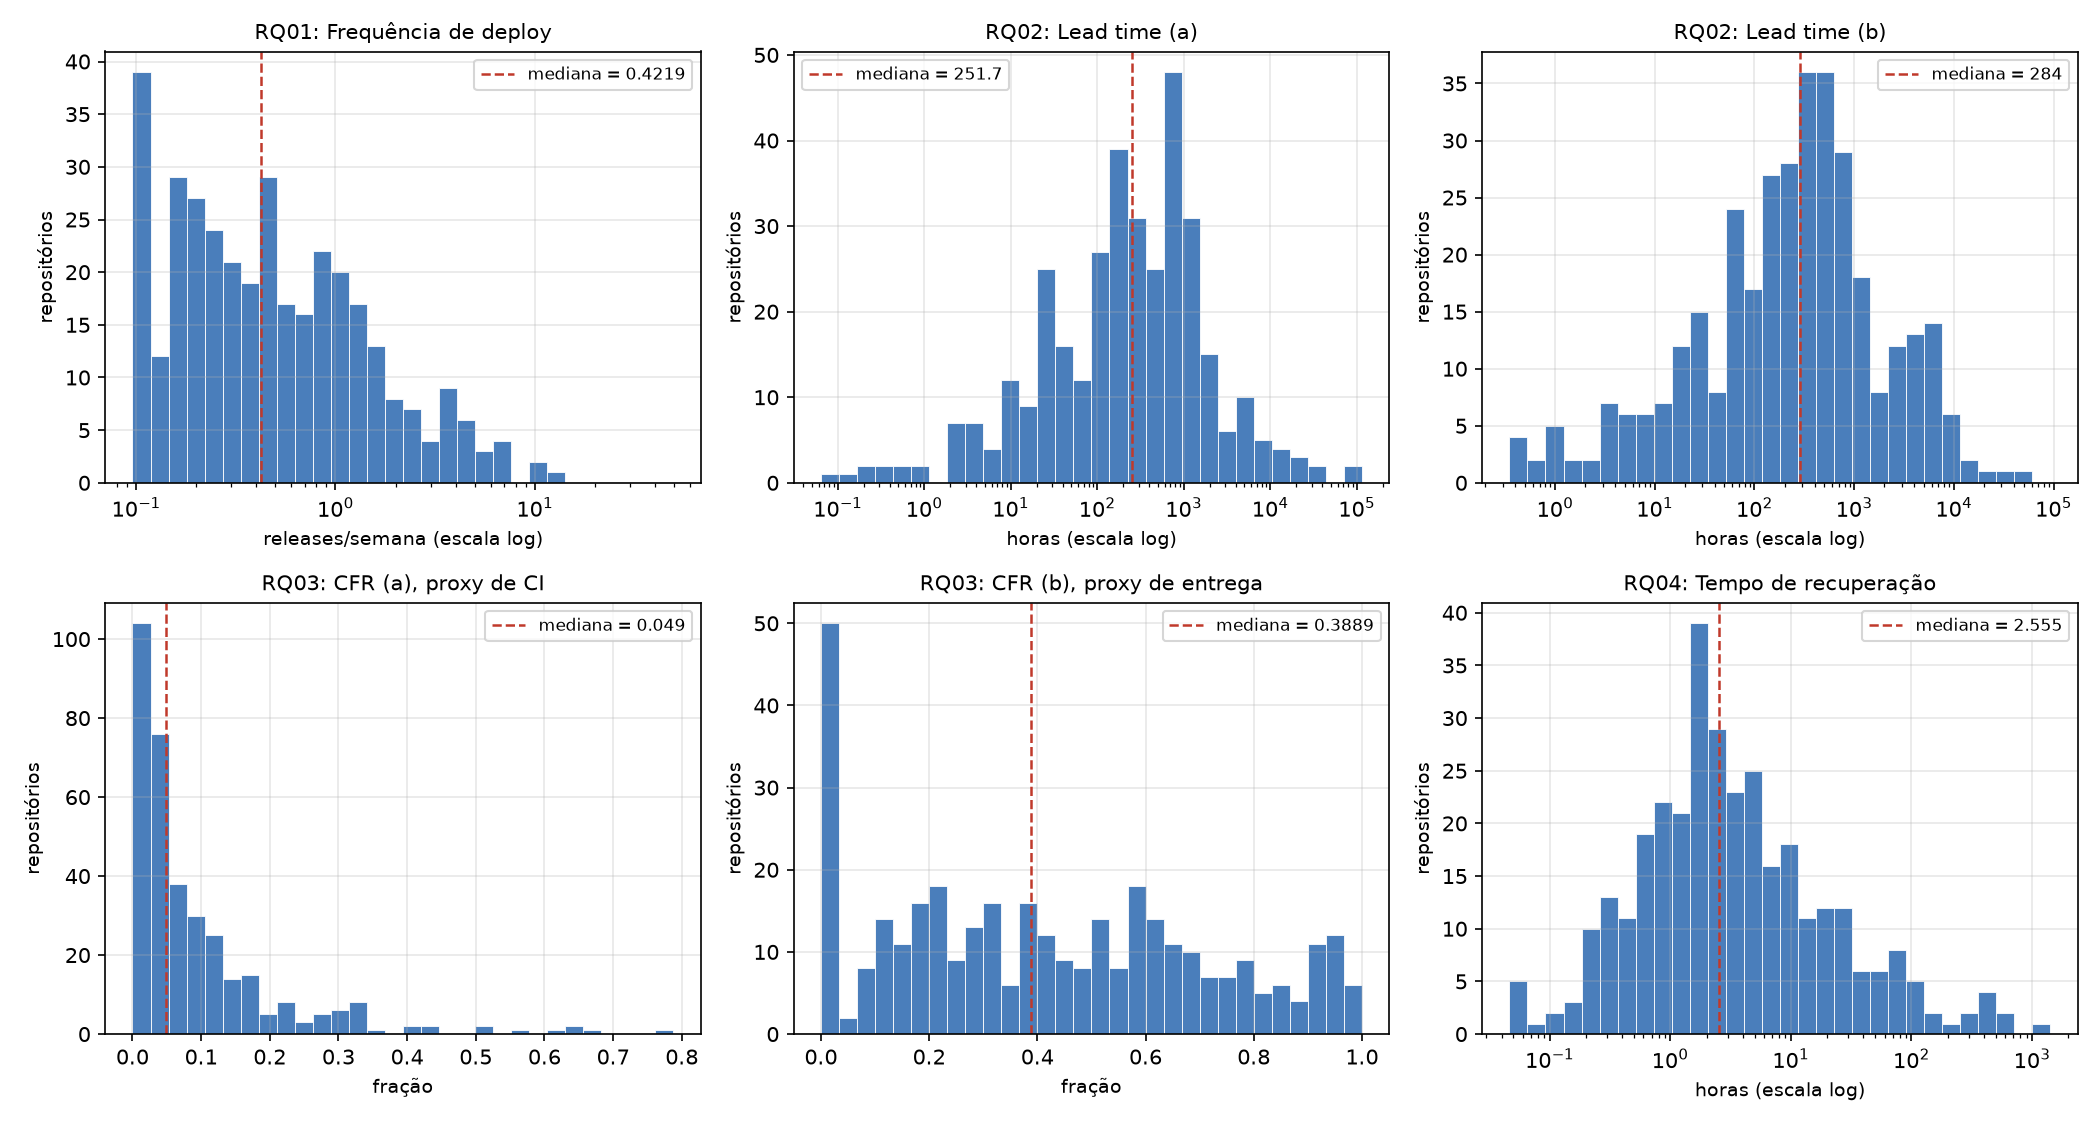
\includegraphics[width=0.92\textwidth]{rq1_rq4_distribuicoes.png}
\caption{Distribuição das seis métricas. Frequência, \textit{lead time} e recuperação em escala
logarítmica; a linha tracejada marca a mediana.}
\label{fig:distribuicoes}
\end{figure}

\textbf{RQ 01.} A mediana é de 0,42 \textit{release} por semana, cerca de uma a cada duas
semanas e meia. 260 repositórios (74,3\%) publicam menos de uma por semana, e só 5 (1,4\%)
alcançam o patamar \textit{Elite} de sete ou mais; 107 (30,6\%) ficam em \textit{Low} e 153
(43,7\%) em \textit{Medium}.

\textbf{RQ 02.} As variantes ficaram próximas: 251,7~h (10,5 dias) na (a) e 284,0~h (11,8
dias) na (b), com ICs quase sobrepostos e correlação de Spearman de 0,744 entre elas. Elas
divergem em repositórios específicos por construção: a variante (a) usa o \textit{commit}
mais antigo de cada \textit{release}, então um único \textit{commit} antigo ``esquecido'' num
ramo faz o \textit{lead time} daquela \textit{release} explodir, enquanto na (b) ele é só um
valor entre muitos e quase não move a mediana. Nas medianas da amostra as duas ficaram
próximas, mas o efeito aparece na cauda: o máximo é de $1{,}1 \times 10^{5}$~h na variante (a)
e de $9{,}3 \times 10^{4}$~h na (b). Pelos cortes
DORA, 57 repositórios ficam em \textit{Elite}, 89 em \textit{High}, 103 em \textit{Medium} e
101 em \textit{Low}.

\textbf{RQ 03.} A mediana do CFR (a) é 0,049 (IQR 0,100), e 13 repositórios (3,7\%) não têm
nenhum \textit{run} com falha; pelos cortes, 283 (80,9\%) ficam em \textit{Elite}. A mediana
do CFR (b) é 0,200 (IQR 0,364), quatro vezes maior, com 80 repositórios (22,9\%) em zero. As
duas variantes ordenam os repositórios de forma muito diferente: a correlação de Spearman
entre elas é de 0,107 ($p = 0{,}045$), e o IC 95\% vai de praticamente zero ($-0{,}0001$) a 0,21.

\textbf{RQ 04.} A mediana é de 2,56~h (IQR 8,55~h) nos 330 repositórios com ao menos um
episódio de falha seguida de sucesso. 196 (59,4\%) ficam em \textit{High} (de 1~h a menos de um
dia), 86 (26,1\%) em \textit{Elite} e 48 (14,5\%) em 24~h ou mais; o máximo é de 1.418~h. Os
20 repositórios (5,7\%) sem nenhum episódio ficam fora da mediana; a maioria deles não teve
falha alguma, como o \texttt{arendst/Tasmota}, com 569 \textit{runs} válidos. A censura foi
desprezível: mediana 0, terceiro quartil 0,0033, e 70,9\% dos repositórios sem nenhum episódio
censurado.

\textbf{Classificação geral.} 25 repositórios (7,1\%) são \textit{Elite}, 143 (40,9\%)
\textit{High}, 159 (45,4\%) \textit{Medium} e 23 (6,6\%) \textit{Low}. A nota de CFR puxa a
categoria para cima (\textit{Elite} em 80,9\% dos casos) e a de frequência para baixo
(\textit{Low} ou \textit{Medium} em 74,3\%).
